\section{Resultados}
\label{section:resultados}


Existem várias métricas que ajudam a definir a capacidade de classificação de um modelo de \emph{deep learning}. Na Seção \ref{section:result-metricas} serão apresentadas as métricas utilizadas, suas expressões e o que elas avaliam. Na Seção \ref{section:result-treinamento}, será comparada a performance do modelo entre o conjunto de treinamento e de validação usando metricas quantitativas. Na Seção \ref{section:result-teste}, os modelos serão avaliados no conjunto de teste usando métricas quantitativas. E, na Seção \ref{section:result-blind}, será feita uma avaliação qualitativa dos modelos no conjunto blind.

\subsection{Métricas de avaliação quantitativa dos modelos}
\label{section:result-metricas}

As métricas aqui utilizadas baseiam-se no erro ou acerto na associação dos objetos às classes pelo modelo. Para relacionar a probabilidade calculada pelo modelo à classe, é definido um limiar de discriminação, que é a probabilidade mínima para que um exemplar pertença à uma classe. Para o cálculo das métricas, foi considerado um de limiar de 0.5.

A primeira métrica apresentada é a acurácia. Ela representa o número de objetos classificados corretamente em relação ao número total de objetos. Sua expressão é mostrada na equação \eqref{eq:acuracia}.

\begin{equation}
  \label{eq:acuracia}
  Acur\acute{a}cia = \frac{TP + TN}{TP + TN + FP + FN}
\end{equation}%
onde $TP$, $TN$, $FP$, e $FN$ são, respectivamente, a quantidade de Verdadeiro Positivo (\emph{True Positive}), Verdadeiro Negativo (\emph{True Negative}), Falso Positivo (\emph{False Positive}) e Falso Negativo (\emph{False Negative}).

Contudo, a acurácia nem sempre é uma métrica confiável para conjunto de dados desbalanceados, pois quanto maior a desproporção do número de objetos entre as classes, menor é o impacto das predições incorretas da classe em minoria no valor da acurácia, levando à uma avaliação superotimista do modelo. Para lidar com isso, usamos outras duas métricas: \emph{Precision} e \emph{Recall}, definidas nas equações \eqref{eq:precisao} e \eqref{eq:recall}, respectivamente.

\begin{equation}
  \label{eq:precisao}
  Precision = \frac{TP}{TP + FP}
\end{equation}

\begin{equation}
  \label{eq:recall}
  Recall = \frac{TP}{TP + FN}
\end{equation}

As equações \eqref{eq:precisao} e \eqref{eq:recall} mostram que $Precision$ tem o valor máximo na ausência de Falso Positivo e $Recall$ tem o valor máximo na ausência de Falso Negativo. Ao adotarmos a classe em minoria como positiva, temos uma avaliação que reflete a capacidade do modelo na tarefa mais difícil -- a classificação correta de objetos na classe com menor representação no conjuto de treinamento.
Para sumarizar estas duas métricas, usamos uma outra, chamada $F_1$\emph{-score}, que é a média harmônica entre $Precision$ e $Recall$, como definida na equação \eqref{eq:f1}.

\begin{equation}
  \label{eq:f1}
  F_1 = 2 \times \frac{Precision \times Recall}{Precision + Recall}
\end{equation}

\newpage
\subsection{Performance dos modelos no treinamento}
\label{section:result-treinamento}



As Figuras \ref{fig:train-metrics} e \ref{fig:val-metrics} mostram avaliações do modelo em cada época de treinamento. A primeira, mostra o valor da custo no próprio conjunto de treinameto e a segunda, mostra o valor da acurácia no conjunto de validação. Na Figura \ref{fig:train-metrics}, notamos que, para a configuração escolhida, ambos os classificadores treinados executam a tarefa de minimizar a função de custo. Mas, para avaliar a capacidade de generalização da rede, ou seja, o potencial de reconhecimento de padrões em um caso real, é importante comparar os resultados com uma amostra diferente do treinamento. O gráfico da acurácia no conjunto de validação (\ref{fig:val-metrics}) mostra que os classificadores e o \emph{Ensemble} conseguem bom desempenho em uma amostra não usada no treinamento.

\begin{figure}[!ht]
  \centering
  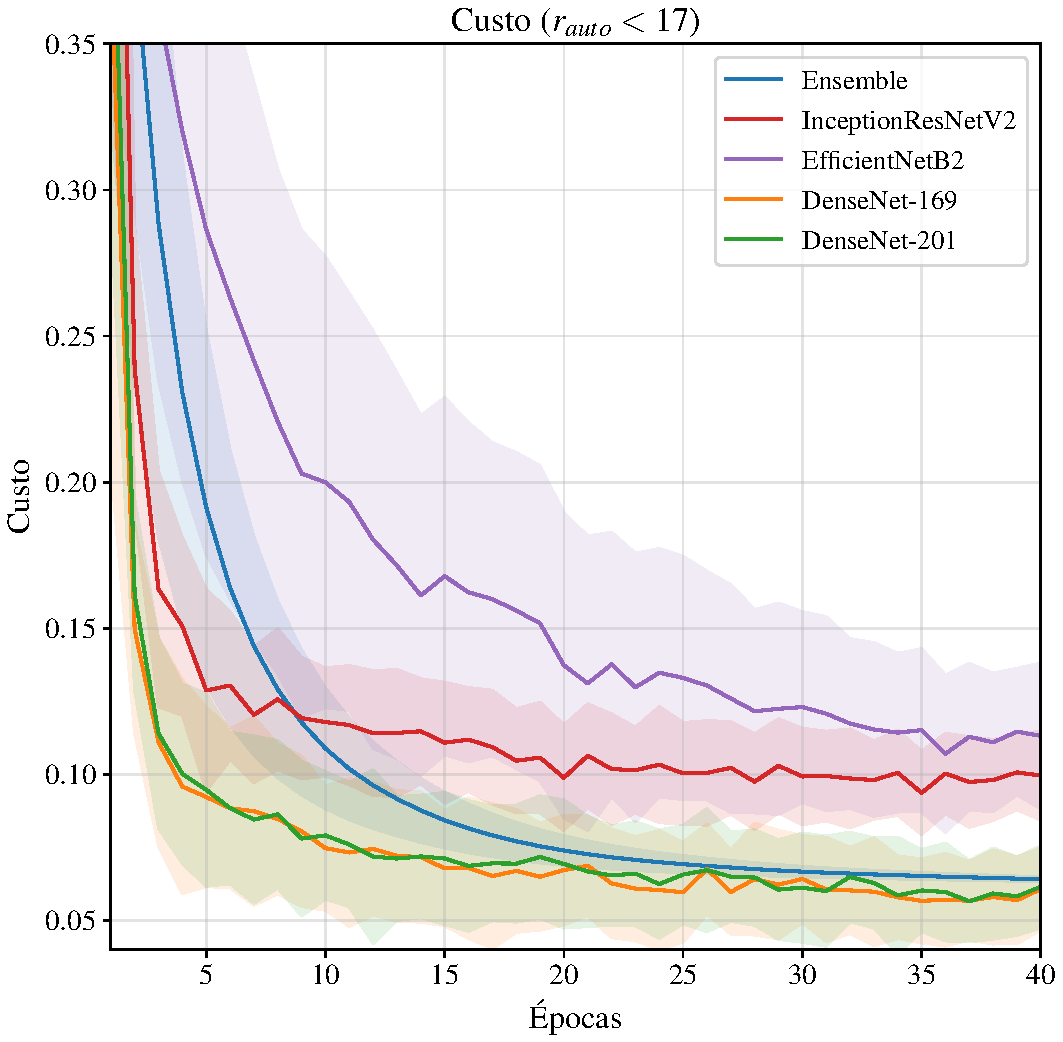
\includegraphics[width=0.82\linewidth]{figures/loss_170.pdf}
  \caption{O gráfico mostra a avialiação dos classificadores individuais e do \emph{Ensemble} no conjunto de treinamento a partir dos valores do custo em função da época de treinamento. As linhas contínuas representam a mediana de 60 medições, enquanto que as regiões sombreadas representam o desvio padrão.}
  \label{fig:train-metrics}
\end{figure}

\begin{figure}[!ht]%
  \centering
  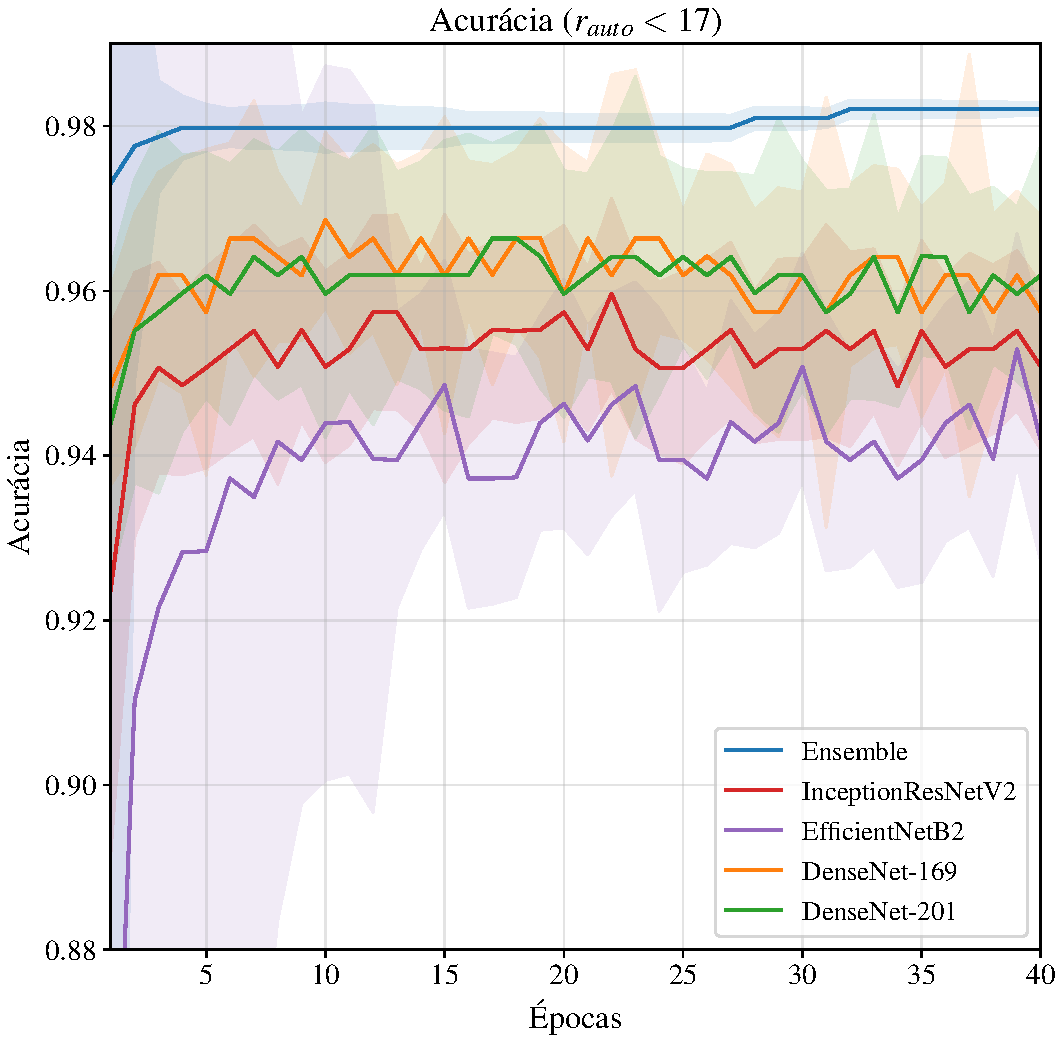
\includegraphics[width=0.82\linewidth]{figures/val_acc_170.pdf}
  \caption{Os gráficos mostram a avaliação dos classificadores individuais e do \emph{Ensemble}. É mostrada a função custo no conjunto de treinamento (em cima) e a acurácia no conjunto de validação (em baixo) para cada época de treinamento. As linhas contínuas representam a mediana de 60 medições, enquanto que as regiões sombreadas representam o desvio padrão.}%
  \label{fig:val-metrics}%
\end{figure}

\clearpage
\newpage
\subsection{Avaliação do modelo no conjunto de teste}
\label{section:result-teste}

\begin{table}[!ht]
  \caption{Avaliação, no conjunto de teste, dos classificadores com os melhores hiperparâmetros.}
  \label{tab:best_hip}
  \centering
  \doubleRuleSep
  \begin{tabular}{l@{\hskip 9pt}*{3}{r@{\hskip 9pt}}r}
    \doubleTopRule
    Parâmetro         & Modelo A          & Modelo B            & Modelo C          & Modelo D          \\
    \midrule
    Arquitetura       & InceptionResNetV2 & EfficientNet-B2     & DenseNet-169      & DenseNet-201      \\
    Learning Rate     & $5\cdot10^{-5}$   & $5\cdot10^{-5}$     & $5\cdot10^{-5}$   & $5\cdot10^{-5}$   \\
    \emph{Batch Size} & 192               & 64                  & 192               & 192               \\
    Amostragem        & \emph{Oversample} & \emph{Class Weight} & \emph{Oversample} & \emph{Oversample} \\
    Optimizador       & NAdam             & Adam                & NAdam             & NAdam             \\
    Unidades          & 512/2             & 256/128/2           & 1024/2            & 1024/2            \\
    \midrule[0.3pt]
    Acurácia (\%)     & $92.75 \pm 0.77$  & $93.12 \pm 0.94$    & $93.12 \pm 0.88$  & $93.48 \pm 0.84$  \\
    $F_1$-Score (\%)  & $96.56 \pm 0.65$  & $96.26 \pm 1.04$    & $97.44 \pm 0.77$  & $97.74 \pm 0.91$  \\
    ROC AUC (\%)      & $97.63 \pm 0.15$  & $97.89 \pm 0.21$    & $97.57 \pm 0.14$  & $97.90 \pm 0.27$  \\
    PR AUC (\%)       & $97.73 \pm 0.14$  & $97.87 \pm 0.30$    & $97.38 \pm 0.20$  & $97.96 \pm 0.30$  \\
    \doubleBottomRule
  \end{tabular}
\end{table}

\begin{table}[!ht]
  \caption{Avaliação, no conjunto de teste, dos classificadores com os melhores hiperparâmetros (redes não utilizadas no \emph{Ensemble}).}
  \label{tab:best_hip2}
  \centering
  \doubleRuleSep
  \begin{tabular}{l@{\hskip 9pt}r@{\hskip 9pt}r}
    \doubleTopRule
    Parâmetro         & Modelo E          & Modelo F          \\
    \midrule
    Arquitetura       & EfficientNet-B7   & VGG16             \\
    Learning Rate     & $5\cdot10^{-5}$   & $1\cdot10^{-5}$   \\
    \emph{Batch Size} & 192               & 192               \\
    Amostragem        & \emph{Oversample} & \emph{Oversample} \\
    Optimizador       & RAdam             & NAdam             \\
    Unidades          & 512/2             & 1024/2            \\
    \midrule[0.3pt]
    Acurácia (\%)     & $91.30 \pm 1.06$  & $93.48 \pm 1.38$  \\
    $F_1$-Score (\%)  & $94.79 \pm 1.02$  & $96.37 \pm 0.97$  \\
    ROC AUC (\%)      & $96.84 \pm 0.19$  & $96.69 \pm 1.14$  \\
    PR AUC (\%)       & $96.94 \pm 0.17$  & $95.85 \pm 1.45$  \\
    \doubleBottomRule
  \end{tabular}
\end{table}

A Tabela \ref{tab:best_hip} sumariza as melhores configurações obtidas para cada uma das arquiteturas utilizadas na construção dos modelos que compõem o \emph{Ensemble} (conforme a Seção \ref{section:classificador}) e suas respectivas avaliações no conjunto de teste. Já a Tabela \ref{tab:best_hip2} sumariza as configurações de outras arquiteturas testadas durante o desenvolvimento mas não colocadas no \emph{Ensemble}. Na parte inferior de ambas as tabelas, foram incluídas as métricas definidas em \ref{section:result-metricas}, para cada classificador, com os melhores hiperparâmetros, como definidos em \ref{section:hyperparam}. Os resultados listados na Tabela \ref{tab:best_hip} mostram a configurações dos classificadores que comporão o \emph{Ensemble}. Os modelos E e F foram não foram incluídos no \emph{Ensemble} por não apresentarem resultados tão bons quanto os demais. A avaliação da rede VGG16 apresenta um alto desvio padrão para todas as métricas e a rede EfficientNetB7 não apresenta resultados compatíveis com o custo computacional.

\begin{figure}[!ht]%
  \centering
  \begin{subfigure}{.61\linewidth}%
    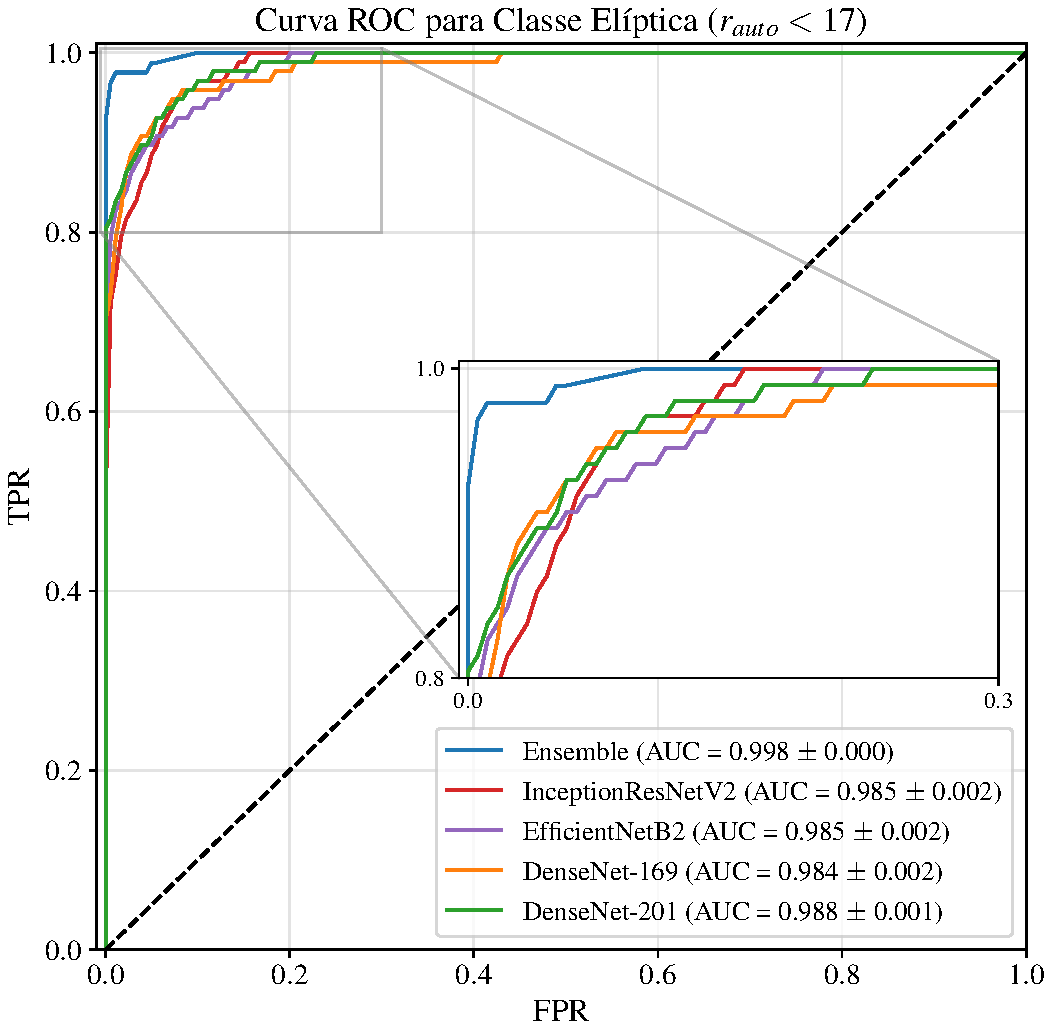
\includegraphics[width=\linewidth]{figures/roc_mn170_E.pdf}
  \end{subfigure}\\[4pt]
  \begin{subfigure}{.61\linewidth}%
    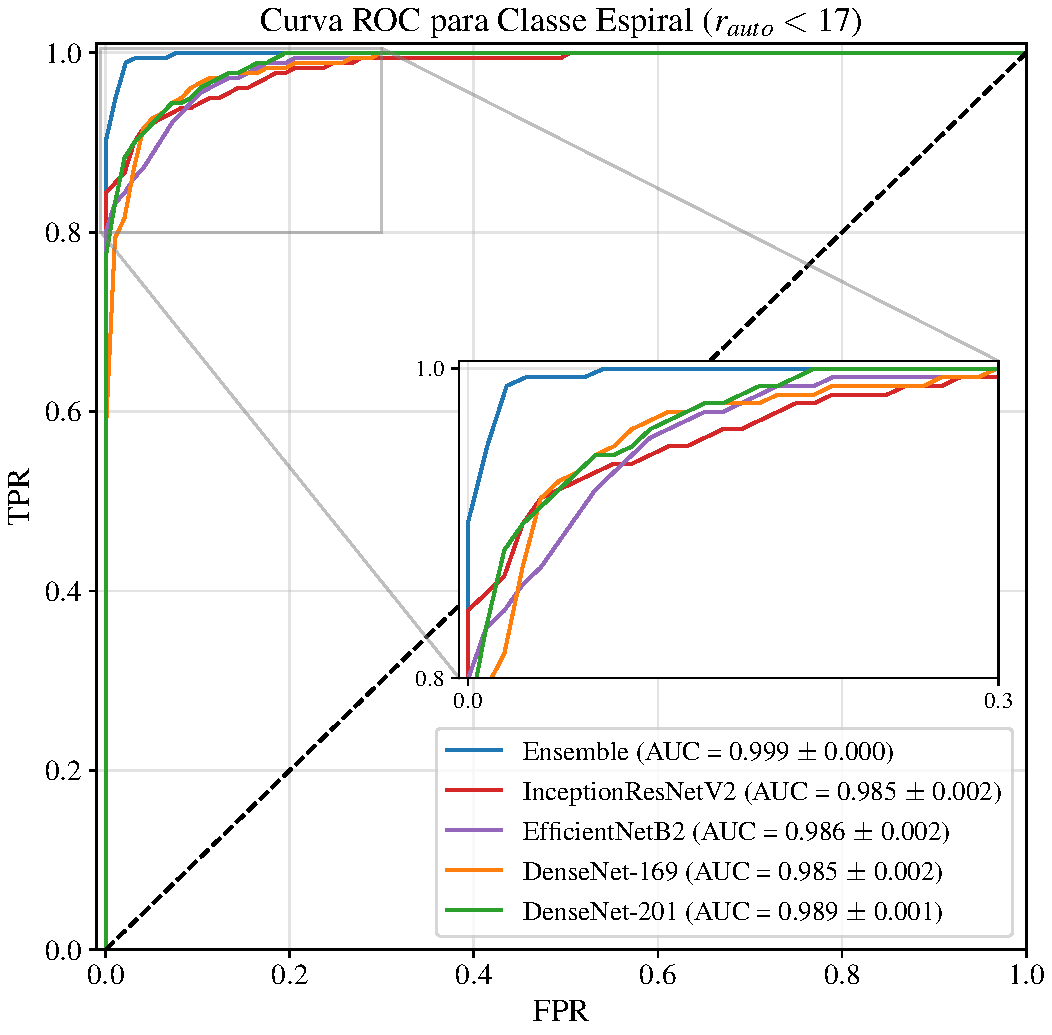
\includegraphics[width=\linewidth]{figures/roc_mn170_S.pdf}
  \end{subfigure}%
  \caption{Curvas ROC dos classificadores individuais e do \emph{Ensemble} separadas pelas classes Elíptica (em cima) e Espiral (em baixo). As linhas contínuas mostram a mediana de 60 curvas e o valor de AUC, na legenda, representa a mediana da área abaixo destas curvas e seu respectivo desvio padrão.}%
  \label{fig:roc}
\end{figure}

\newpage

\begin{figure}[!ht]%
  \centering
  \begin{subfigure}{.62\linewidth}%
    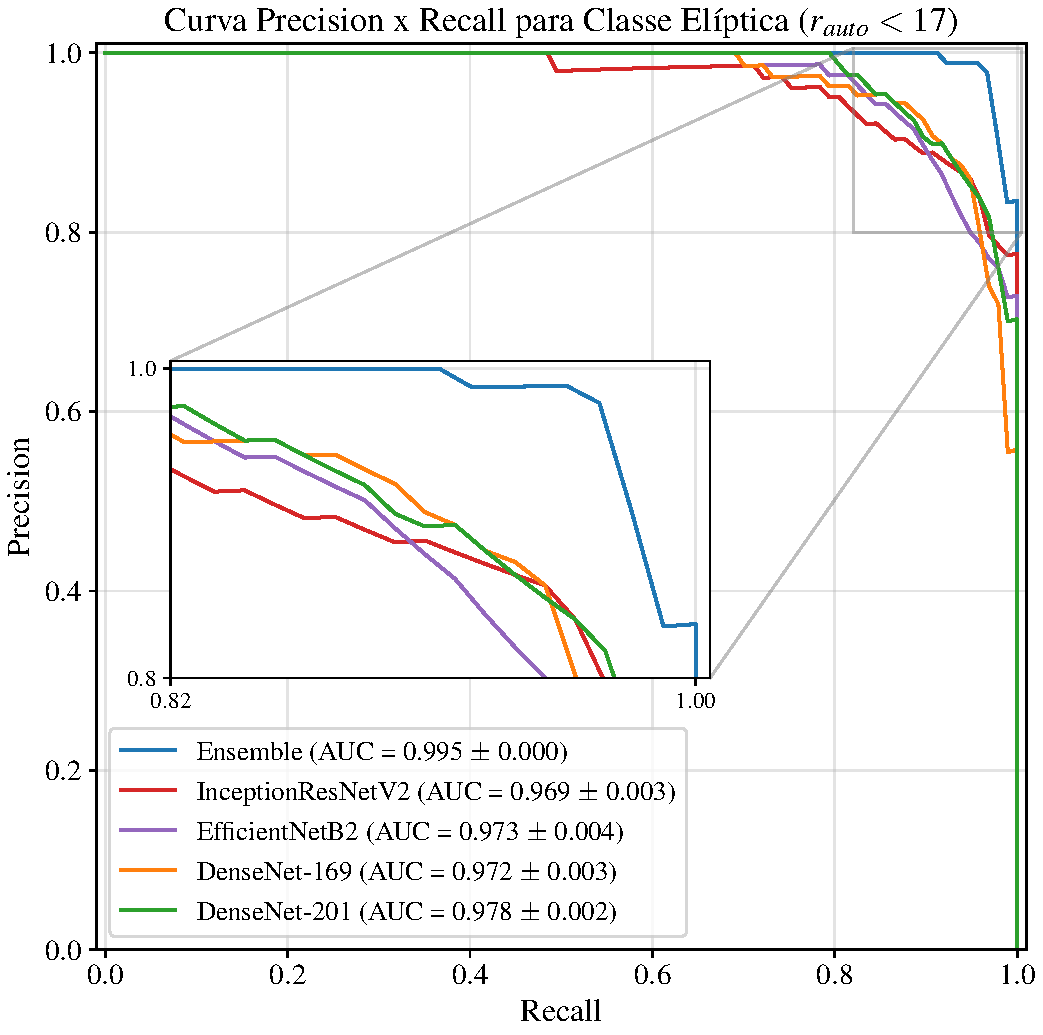
\includegraphics[width=\linewidth]{figures/pr_mn170_E.pdf}
  \end{subfigure}\\[4pt]
  \begin{subfigure}{.62\linewidth}%
    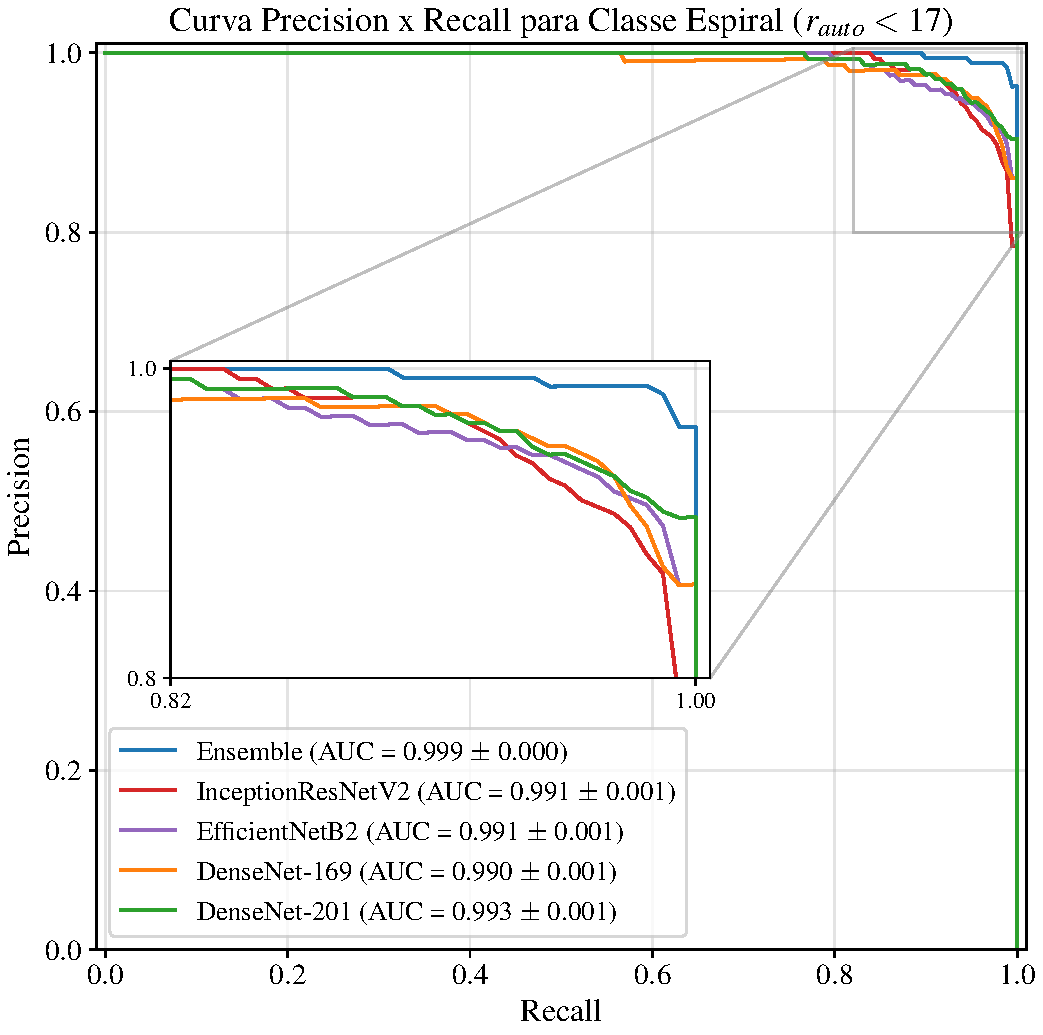
\includegraphics[width=\linewidth]{figures/pr_mn170_S.pdf}
  \end{subfigure}%
  \caption{Curvas \emph{Precision x Recall} dos classificadores individuais e do \emph{Ensemble} separadas pelas classes Elíptica (em cima) e Espiral (em baixo). As linhas contínuas mostram a mediana de 60 curvas e o valor de AUC, na legenda, representa a mediana da área abaixo destas curvas e seu respectivo desvio padrão.}%
  \label{fig:pr}
\end{figure}

\begin{table}[!ht]
  \centering
  \caption{Sumário das métricas de avaliação do \emph{Ensemble} (Seção \ref{section:meta-modelo}) no conjunto de teste.}
  \label{tab:ensemble}
  \doubleRuleSep
  \begin{tabular}{lr}
    \doubleTopRule
    Métrica     & Valor (\%)       \\
    \midrule[0.3pt]
    Acurácia    & $98.52 \pm 0.13$ \\
    $F_1$-Score & $98.52 \pm 0.13$ \\
    ROC AUC     & $99.81 \pm 0.01$ \\
    PR AUC      & $99.82 \pm 0.01$ \\
    \doubleBottomRule
  \end{tabular}
\end{table}




A Tabela \ref{tab:ensemble} mostra os resultados para o \emph{Ensemble}, obtido ao se combinar os modelos de A a D, como descrito na Seção \ref{section:meta-modelo}. Outra análise, mais robusta do que é mostrado nessa tabela, é avaliar os modelos sob diferentes limiares de discriminação, ao invés de sob apenas um. Para isto, usamos a Curva Característica de Operação do Receptor \emph{(Receiver Operating Characteristic -- ROC)} \cite{Hanley1982,Fawcett2006}, que é um gráfico de $FPR$ (False Positive Rate) versus $TPR$ (True Positive Rate). Usamos também a \emph{Curva Precision-Recall} (PR) que é um diagnóstico pontente para avaliar a classificação de modelos treinados a partir de conjuntos de dados desbanlanceados, como é o caso aqui.

A curva ROC pode ser visualizadas na Figura \ref{fig:roc}, onde resultados para os modelos individuais e para o Emsemble são comparados.
Note que a curva ROC é tão melhor quanto maior for a área abaixo desta (\emph{Area Under Curve -- AUC}), pois essa área representa o grau de separabilidade de um modelo. Na Figura \ref{fig:pr} mostramos a curva PR e o mesmo comentário vale aqui sobre o AUC. Fica claro ao analisar ambas as Figuras \ref{fig:roc} e \ref{fig:pr},  que os resultados do Emsemble são claramente melhores, AUC maiores.

\newpage

\subsection{Avaliação do modelo no conjunto blind}
\label{section:result-blind}

\begin{figure}[!ht]%
  \centering
  \begin{subfigure}{.57\linewidth}
    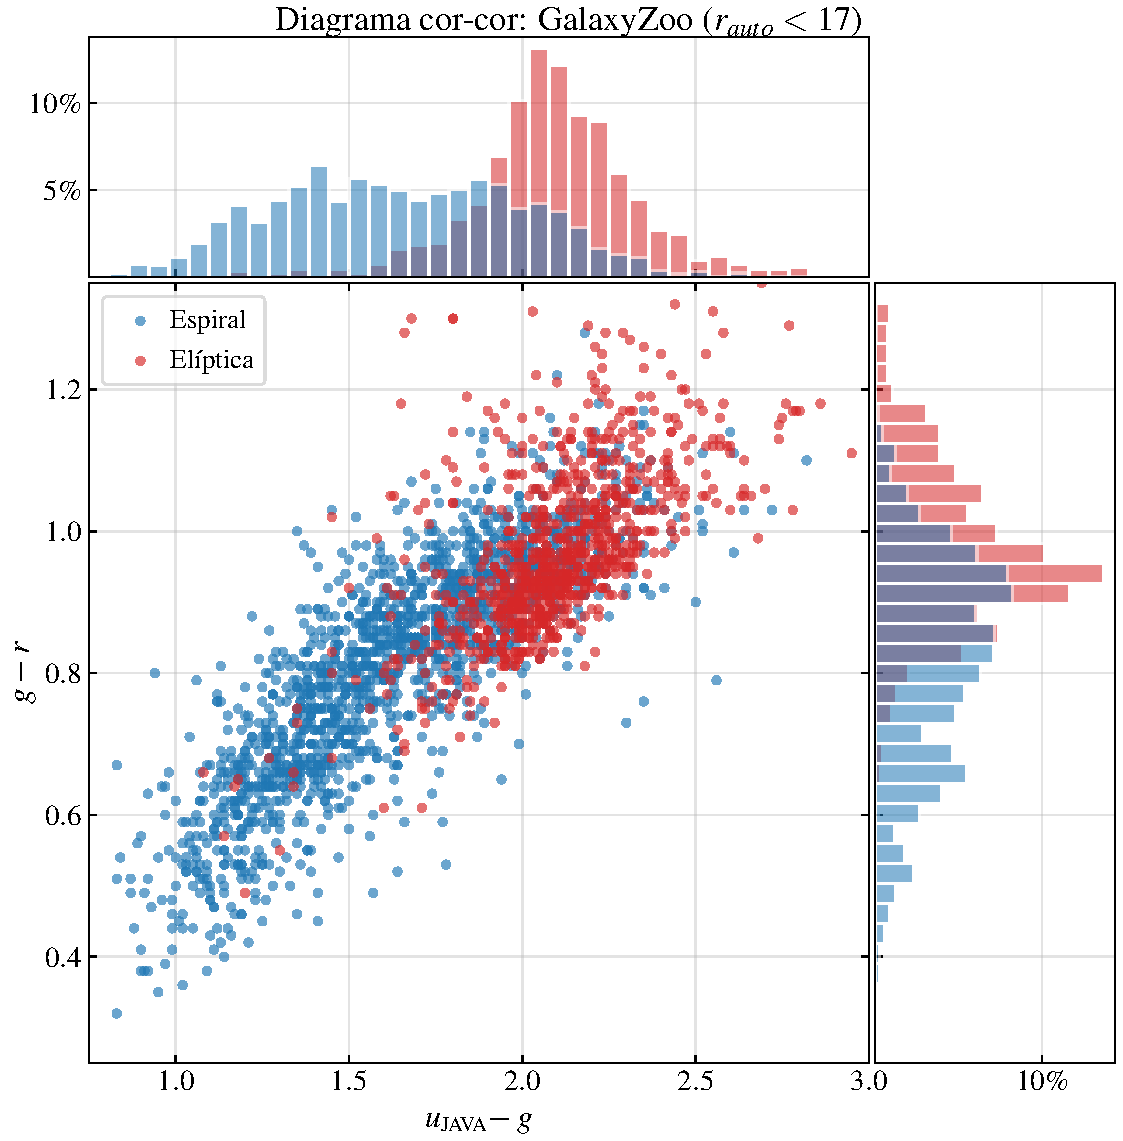
\includegraphics[width=\linewidth]{figures/zoo170_color_color.pdf}
  \end{subfigure}\\[4pt]
  \begin{subfigure}{.57\linewidth}
    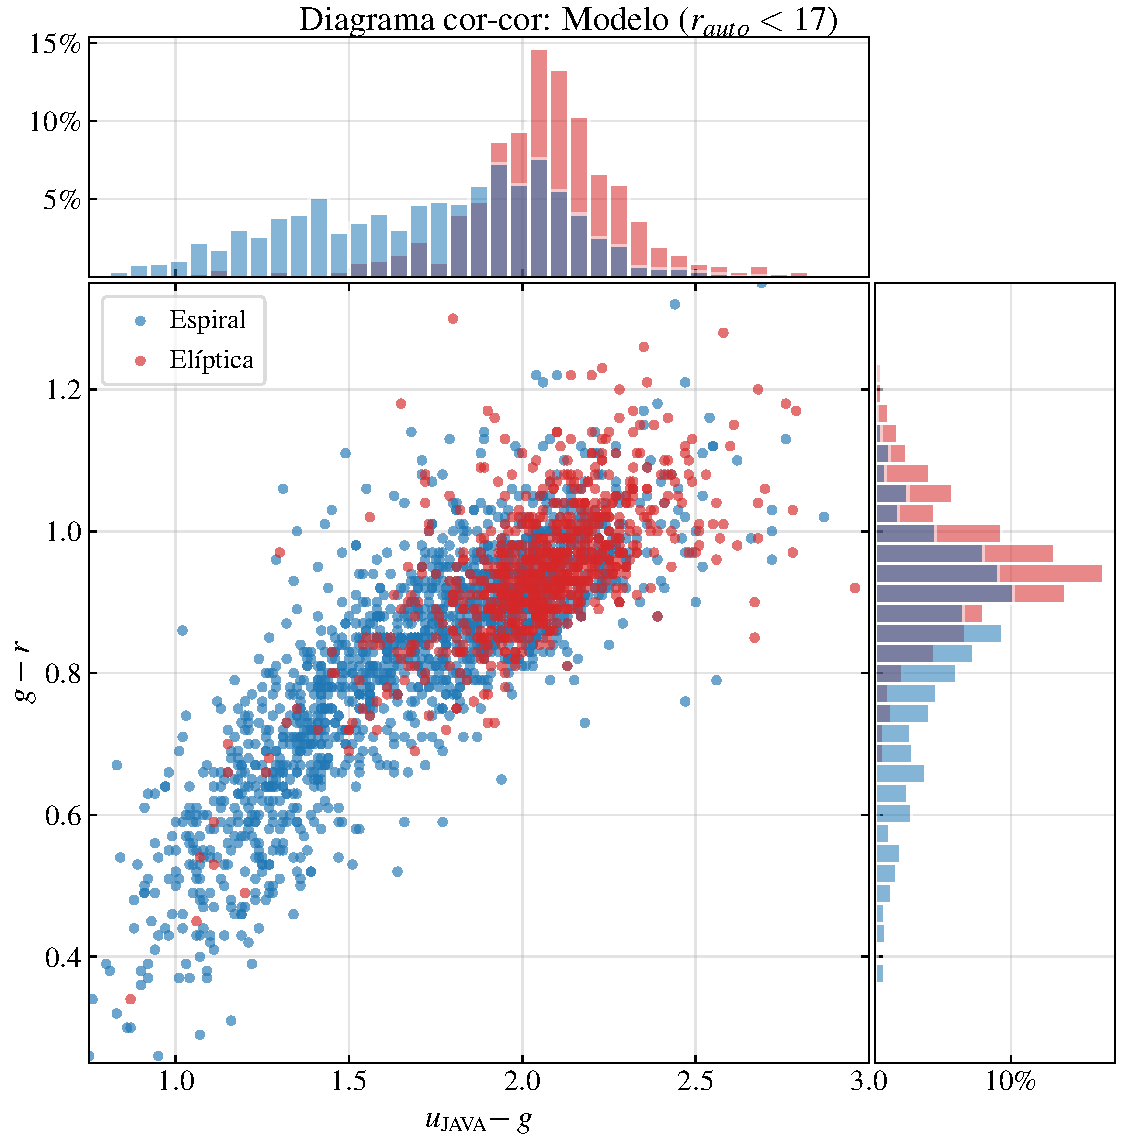
\includegraphics[width=\linewidth]{figures/mn170_color_color.pdf}
  \end{subfigure}
  \caption{Diagrama cor-cor de $u_{JAVA} - g$ versus $g - r$. Em cima, classificações visuais do GalaxyZoo nos conjuntos de treino, validação e teste e, em baixo, classificações na amostra Blind feitas pelos modelos treinados. Em azul, galáxias classificadas como Espirais e, em vermelho, galáxias classificadas como Elípticas.}%
  \label{fig:color-color}%
\end{figure}

Um dos objetivos deste trabalho é obter classificações de galáxias elípticas e espirais, que não foram ainda classificadas (nas chamadas amostras \emph{blind}). Isto foi feito para uma amostra contendo 2536 galáxias com magnitude $r_{auto} < 17$, com distribuições de magnitude e redshift compatíveis com as amostras de treinamento, como mostrado na Seção \ref{section:divisao_conjunto_de_dados}.

Uma maneira mais qualitativa de avaliar os resultados da classificação é pela análise do diagrama cor-cor das galáxias, comparando as nossas classificações com a do Galaxy Zoo. Nesta análise, é muito importante lidar com  amostras com distribuições de magnitude e redshift similares, como visto na Seção \ref{section:divisao_conjunto_de_dados}.

A Figura \ref{fig:color-color} mostra um diagrama de $u_{JAVA} - g$ versus $g - r$. Os painéis da esquerda mostram classificações visuais obtidas do GalaxyZoo nos conjuntos de treino, validação e teste enquanto que os painéis da direita mostram classificações feitas pelos nossos modelos descritos neste trabalho, no conjunto Blind. Como esta comparação é feita entre amostras diferentes de galáxias (embora com distribuição de brilho e redshift similares), não é esperado que os gráficos da esquerda sejam idênticos aos da direita, mas que tenham formas parecidas. Logo, o que se pretende mostrar é que a semelhança entre os diagramas da classificação humana com a classificação automática (usando nosso modelo) é um indicativo de uma classificação robusta.

As Figuras \ref{fig:grid-s1} e \ref{fig:grid-s2} mostram duas amostras aleatórias do conjunto \emph{blind} de galáxias classificadas como espiral ($P_S > 0.5$) pelo modelo. Enquanto que as Figuras \ref{fig:grid-e1} e \ref{fig:grid-e2} mostram duas amostras aleatórias do conjunto \emph{blind} de galáxias classificadas como elípticas ($P_E > 0.5$) pelo modelo.

\newpage

\begin{figure}[!ht]
  \centering
  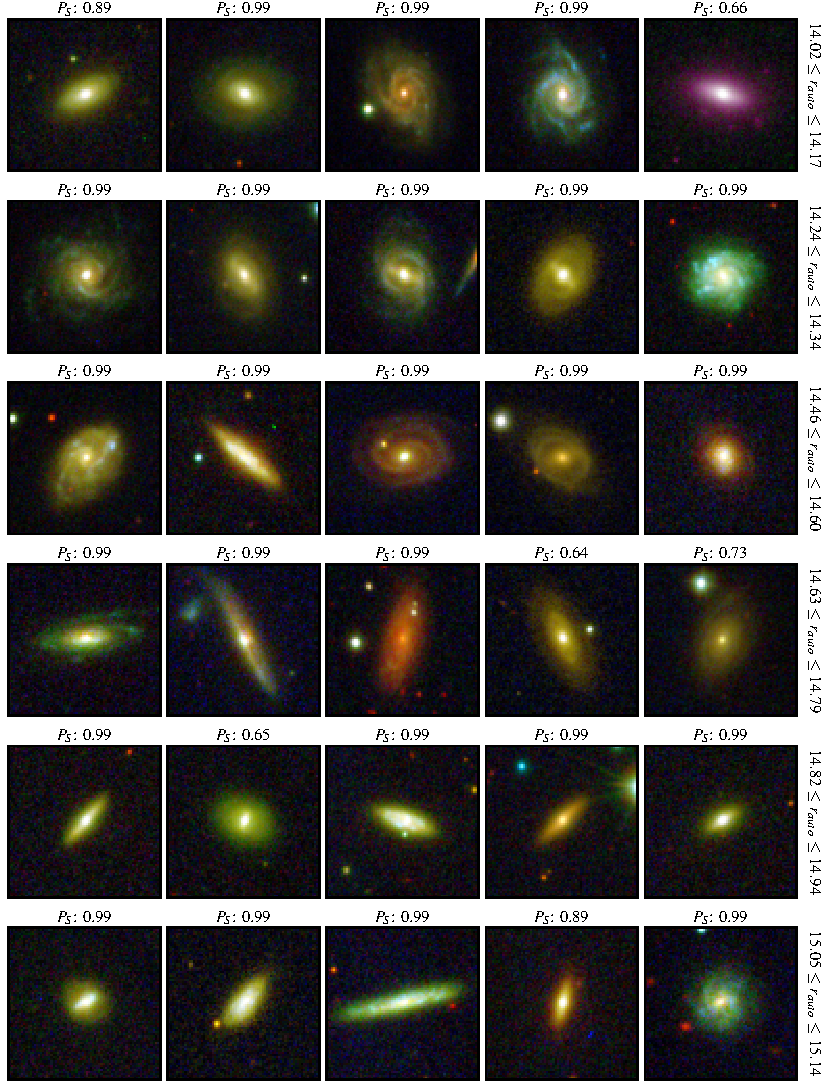
\includegraphics[width=0.95\linewidth]{figures/blind_preds_spir_1.pdf}
  \caption{Amostra aleatória de 30 galáxias do conjunto \emph{blind} com classificações dadas pelo modelo proposto dispostas em ordem crescente de magnitude $r_{auto}$. O valor de $P_S$ mostra a probabilidade da galáxia pertencer à classe espiral.}
  \label{fig:grid-s1}
\end{figure}

\begin{figure}[!ht]
  \centering
  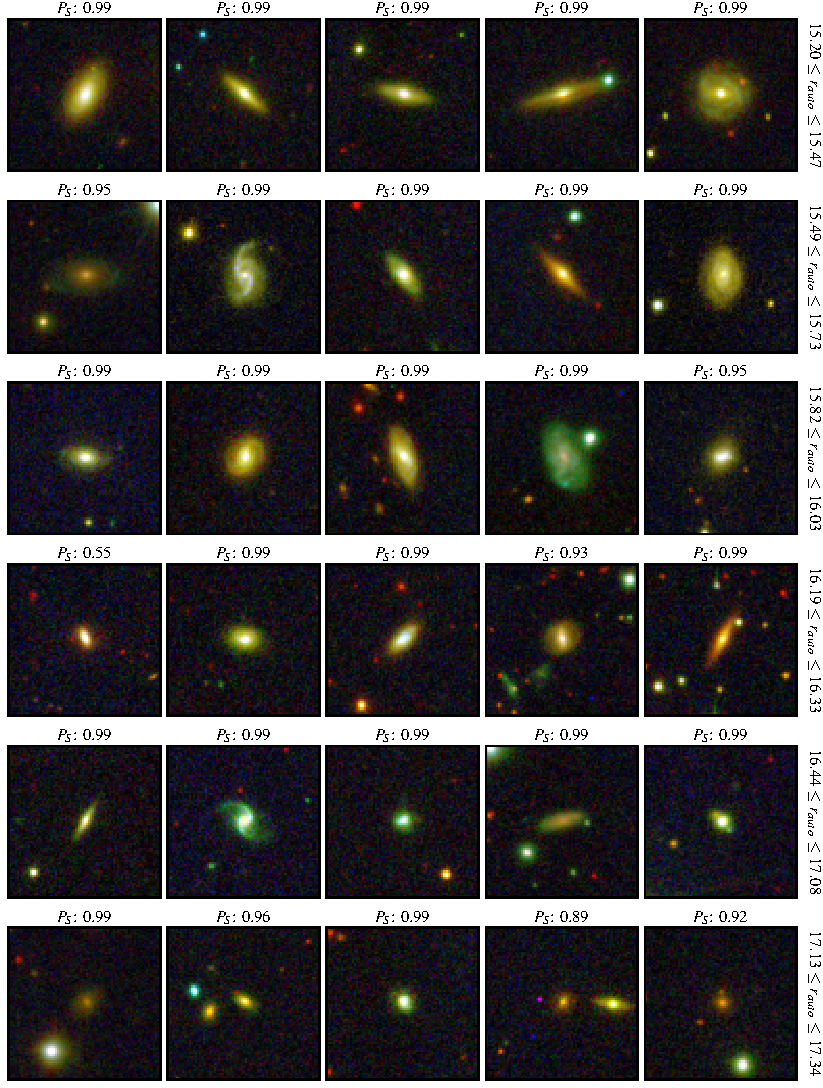
\includegraphics[width=0.95\linewidth]{figures/blind_preds_spir_2.pdf}
  \caption{Amostra aleatória de 30 galáxias do conjunto \emph{blind} com classificações dadas pelo modelo proposto dispostas em ordem crescente de magnitude $r_{auto}$. O valor de $P_S$ mostra a probabilidade da galáxia pertencer à classe espiral.}
  \label{fig:grid-s2}
\end{figure}

\begin{figure}[!ht]
  \centering
  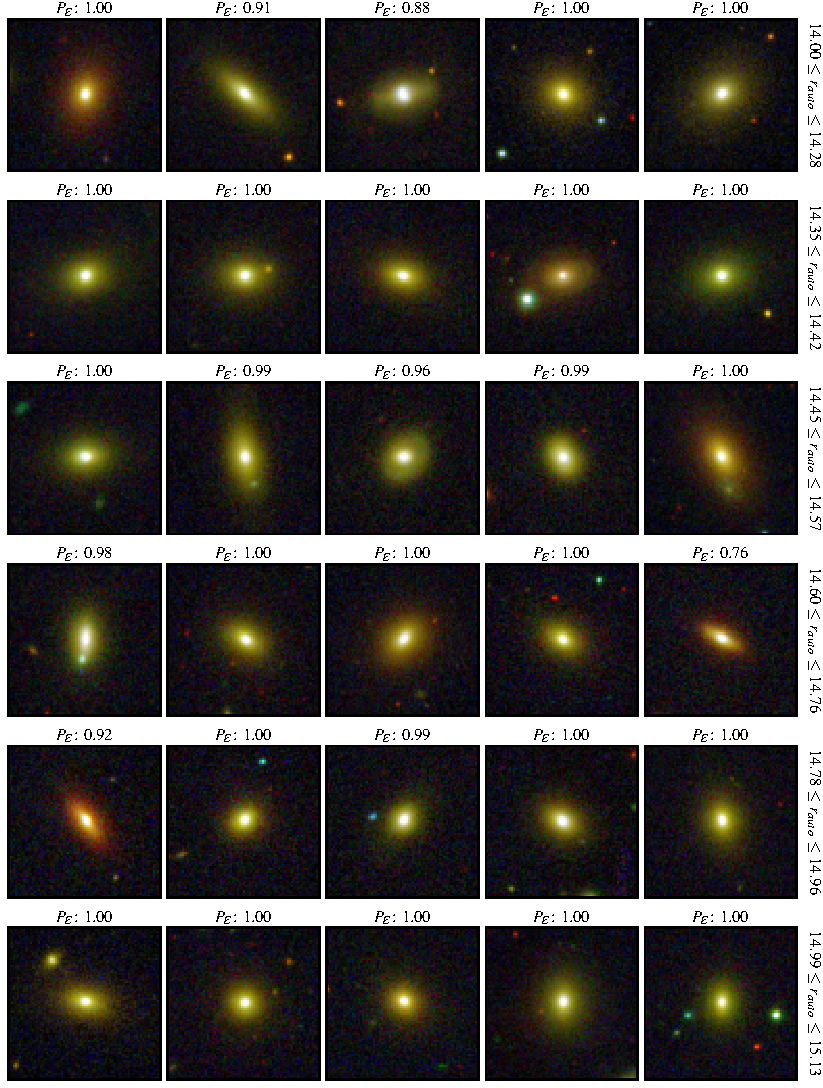
\includegraphics[width=0.95\linewidth]{figures/blind_preds_ellip_1.pdf}
  \caption{Amostra aleatória de 30 galáxias do conjunto \emph{blind} com classificações dadas pelo modelo proposto dispostas em ordem crescente de magnitude $r_{auto}$. O valor de $P_E$ mostra a probabilidade da galáxia pertencer à classe elíptica.}
  \label{fig:grid-e1}
\end{figure}

\begin{figure}[!ht]
  \centering
  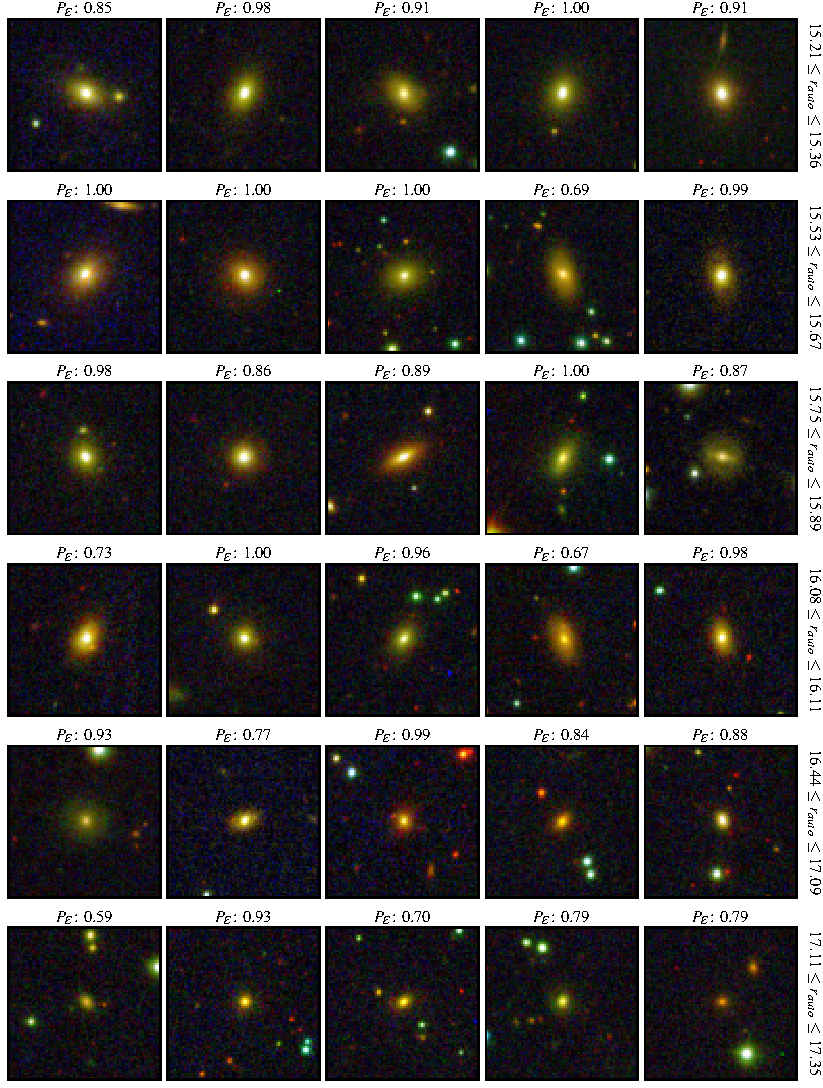
\includegraphics[width=0.95\linewidth]{figures/blind_preds_ellip_2.pdf}
  \caption{Amostra aleatória de 30 galáxias do conjunto \emph{blind} com classificações dadas pelo modelo proposto dispostas em ordem crescente de magnitude $r_{auto}$. O valor de $P_E$ mostra a probabilidade da galáxia pertencer à classe elíptica.}
  \label{fig:grid-e2}
\end{figure}